\documentclass[11pt,aspectratio=169,dvipsnames]{beamer}
\graphicspath{{figs/}}
\usetheme{default}
\usepackage{DasBeamerPaket}
\usepackage{animate}
\usepackage{lastpage}
\usepackage{tikz}
\usepackage[normalem]{ulem}

\setbeamercolor{section in toc}{fg=NavyBlue}
\setbeamercolor{frametitle}{fg=NavyBlue}
\captionsetup[figure]{labelfont=bf}
\captionsetup[table]{labelfont=bf}
\newcommand{\theauthor}{Jakob Krause}
\newcommand{\theshortauthor}{J. Krause}
\newcommand{\authormail}{krause@hiskp.uni-bonn.de}
\newcommand{\authorgit}{krausejm}
\newcommand{\thetitle}{$\Sigma$ in $\gamma p \to p \eta^{(_{'})}\to p\gamma\gamma$}
\newcommand{\thecolor}{black!70!blue}
\newcommand{\thesubtitle}{Master thesis for the CBELSA/TAPS collaboration}
\newcommand{\thedate}{18th January 2022}
\begin{document}
	\definecolor{myWhite}{rgb}{1,1,1}
	\setbeamertemplate{footline}[text line]{\parbox{\linewidth}{\vspace*{-9pt}\textcolor{white}{\textsc{\theshortauthor}  \hfill\thetitle\hfill}\textcolor{myWhite}{\insertpagenumber/\pageref{LastPage}}}}
	\addtobeamertemplate{footline}{ \makebox[0pt][l]{\hspace{-1cm}
			\raisebox{0cm}[0pt][0pt]{\colorbox{\thecolor}{\phantom{{\large TEXTTEXTTEXTTEXTTEXTTEXTTEXTTEXTTEXTTEXTTEXTTEXTTEXTTEXTTEXTTEXTTEXTTEXTTEXTTEXTTEXTTEXTTEXTTEXTTEXTTEXTTEXTTEXTTEXTTEXTTEXTTEXTTEXTTEXTTEXTTEXTTEXTTEXTTEXTTEXT}}}}}}
	
	\setbeamercovered{transparent}
	\setbeamertemplate{navigation symbols}{}
	\setbeamertemplate{frametitle}[default][left,leftskip=0.5cm]
	\setbeamertemplate{itemize item}{\color{black}$\blacktriangleright$}
	\setbeamertemplate{section in toc}[sections numbered]
	\setbeamercolor{section in toc}{fg=\thecolor}
	\setbeamercolor{frametitle}{fg=\thecolor}
	\captionsetup{font=scriptsize,labelfont=scriptsize}
	\AtBeginSection[]
	{	
		\definecolor{myWhite}{rgb}{0,0,0}
		\begin{frame}[noframenumbering]
			\frametitle{}
			\addtocounter{page}{-1}
			\tableofcontents[currentsection]
			
		\end{frame}
		\definecolor{myWhite}{rgb}{1,1,1}
	}
\begin{frame}{\textsc{Bayesian} fit of event yield asymmetries}
\textsc{Markov}-Chain diagnostics:
\begin{itemize}
\item \textsc{Monte-Carlo} Standard-Error (MCSE)
\item $\hat{R}$
\end{itemize}
Goodness of Fit:
\begin{itemize}
	\item $p$-value calculated from reproduced data
\end{itemize}
\end{frame}
	\begin{frame}{\textsc{Bayesian} fit of event yield asymmetries}
		\begin{figure}
			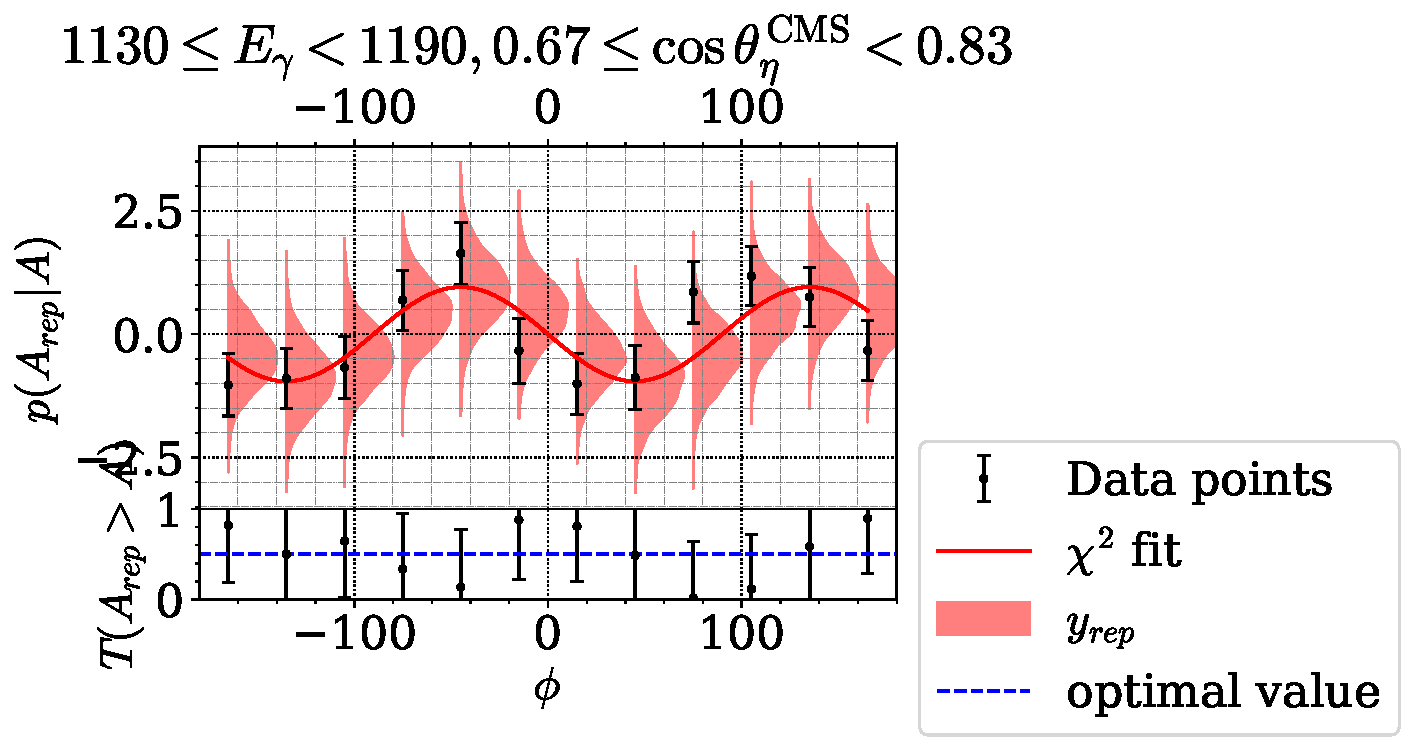
\includegraphics[width=\linewidth]{../../bayes/realdeal/ppd_checks/ebin0costbin10.pdf}
		\end{figure}
	\end{frame}
	\begin{frame}{\textsc{Bayesian} fit of event yield asymmetries}
		\begin{figure}
			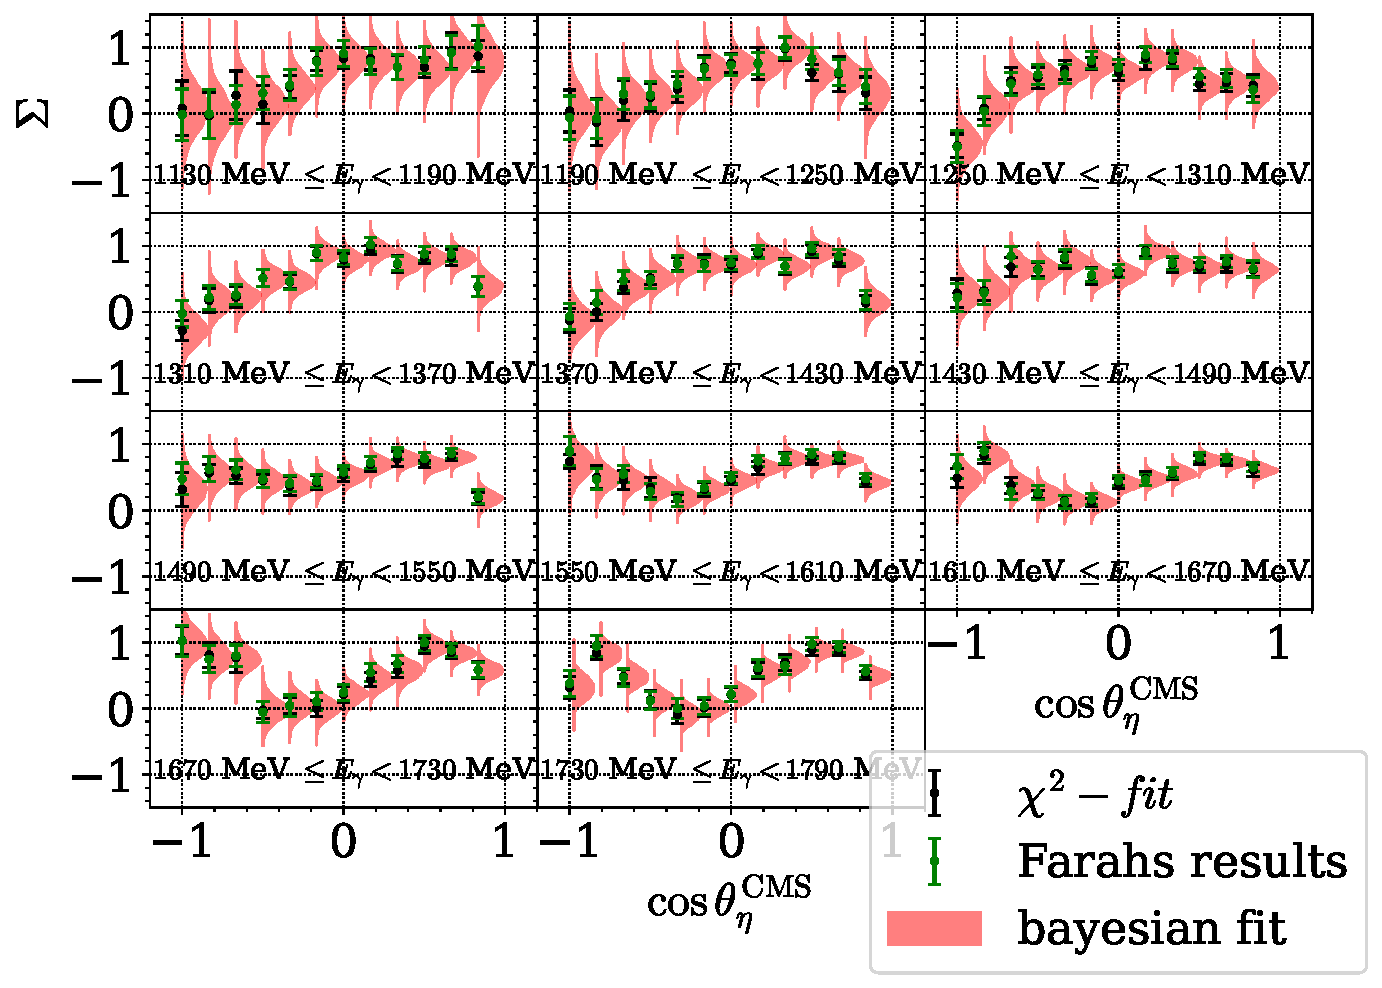
\includegraphics[width=.8\linewidth]{../../bayes/realdeal/sigma_eta.pdf}
		\end{figure}
	\end{frame}
	
	\begin{frame}{Event selection}
		2013 hydrogen beam time
		\begin{itemize}
			\item charge cut (3 PED)
			\item time cuts (prompt peak and bkg substraction)
			\item $E_\gamma > 1400$ MeV
			\item\sout{$E_\gamma^\text{calc}>1447$ MeV}
			\item coplanarity
			\item polar angle
			\item missing mass
			\item  invariant mass
		\end{itemize}
	\end{frame}

\begin{frame}{Event selection}
	\begin{figure}
		\centering
		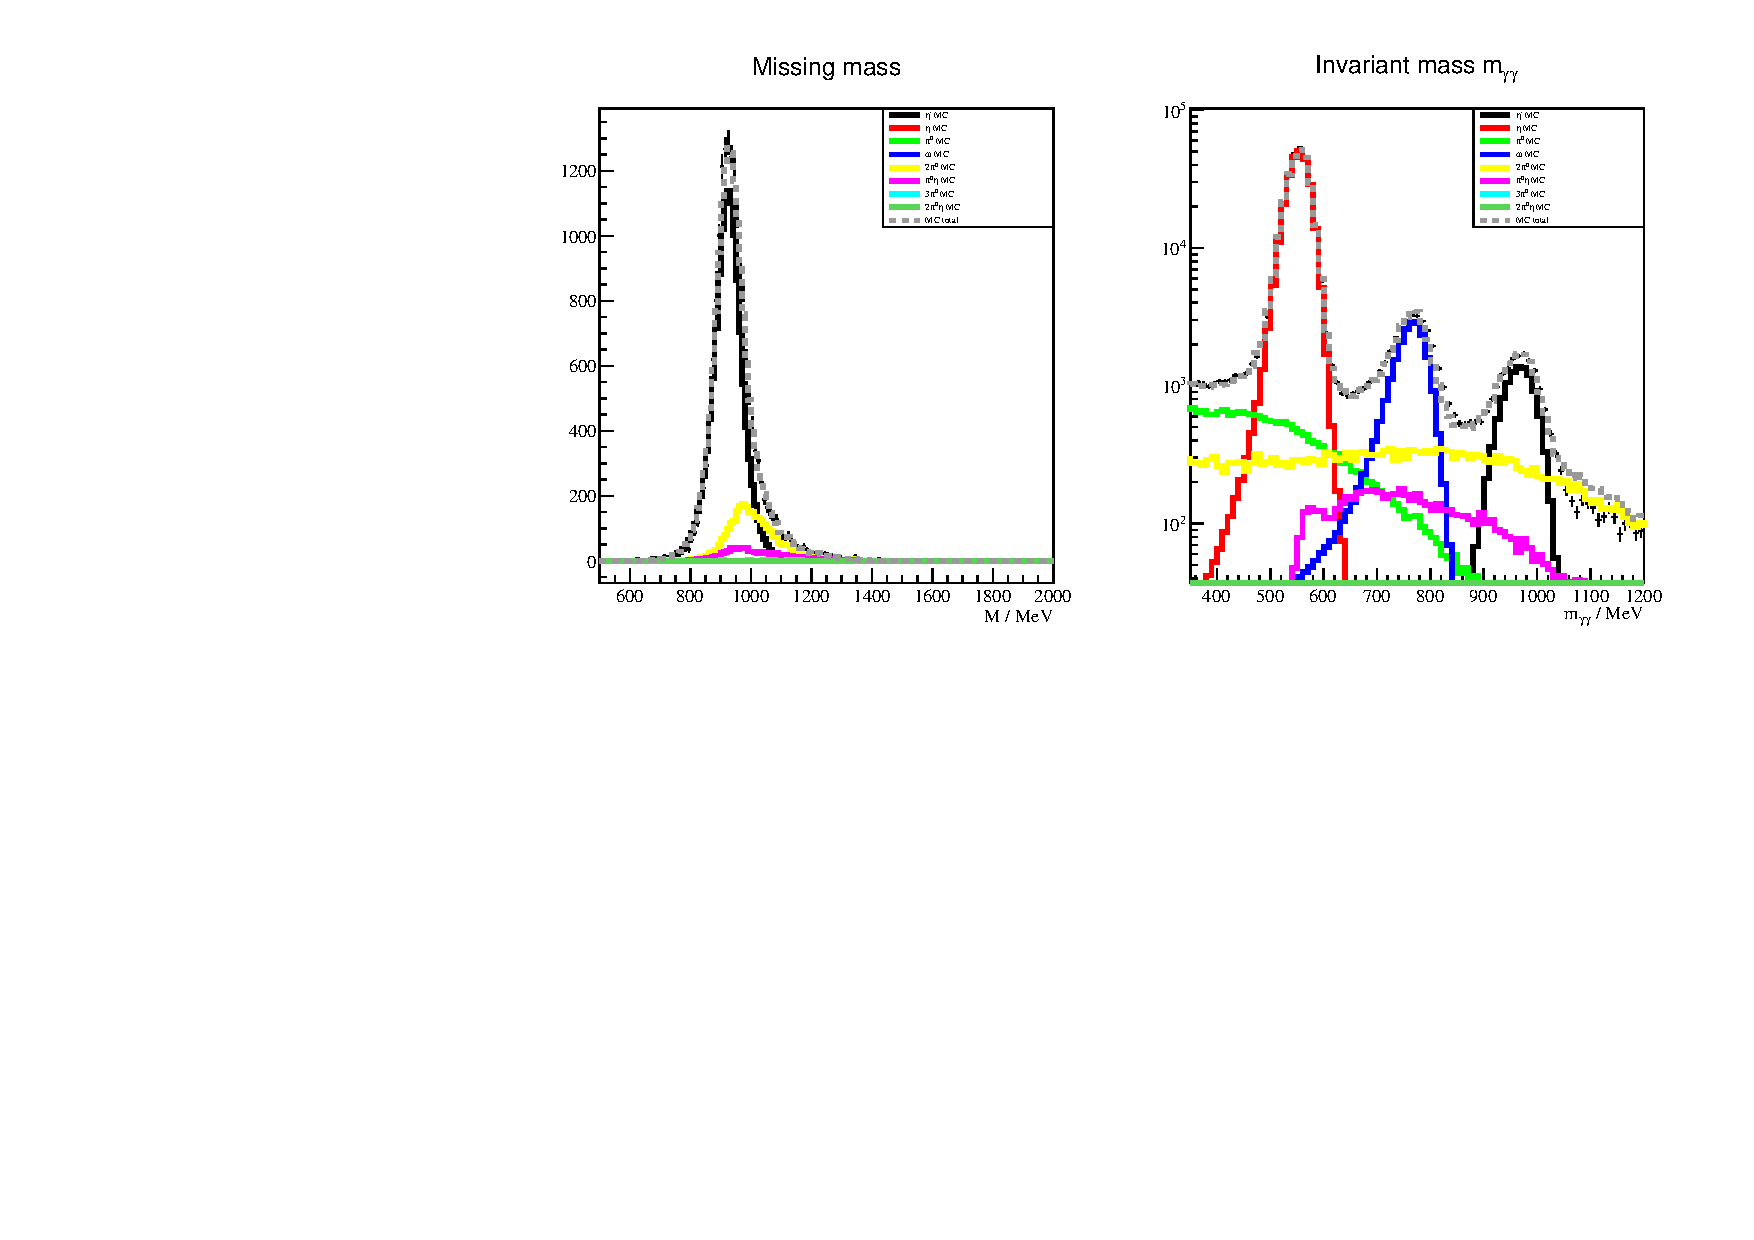
\includegraphics[width=\linewidth]{../../figs/hydrogen/global_mism_inv.pdf}
	\end{figure}
\end{frame}
	\begin{frame}{Event selection}
		\begin{figure}
			\centering
			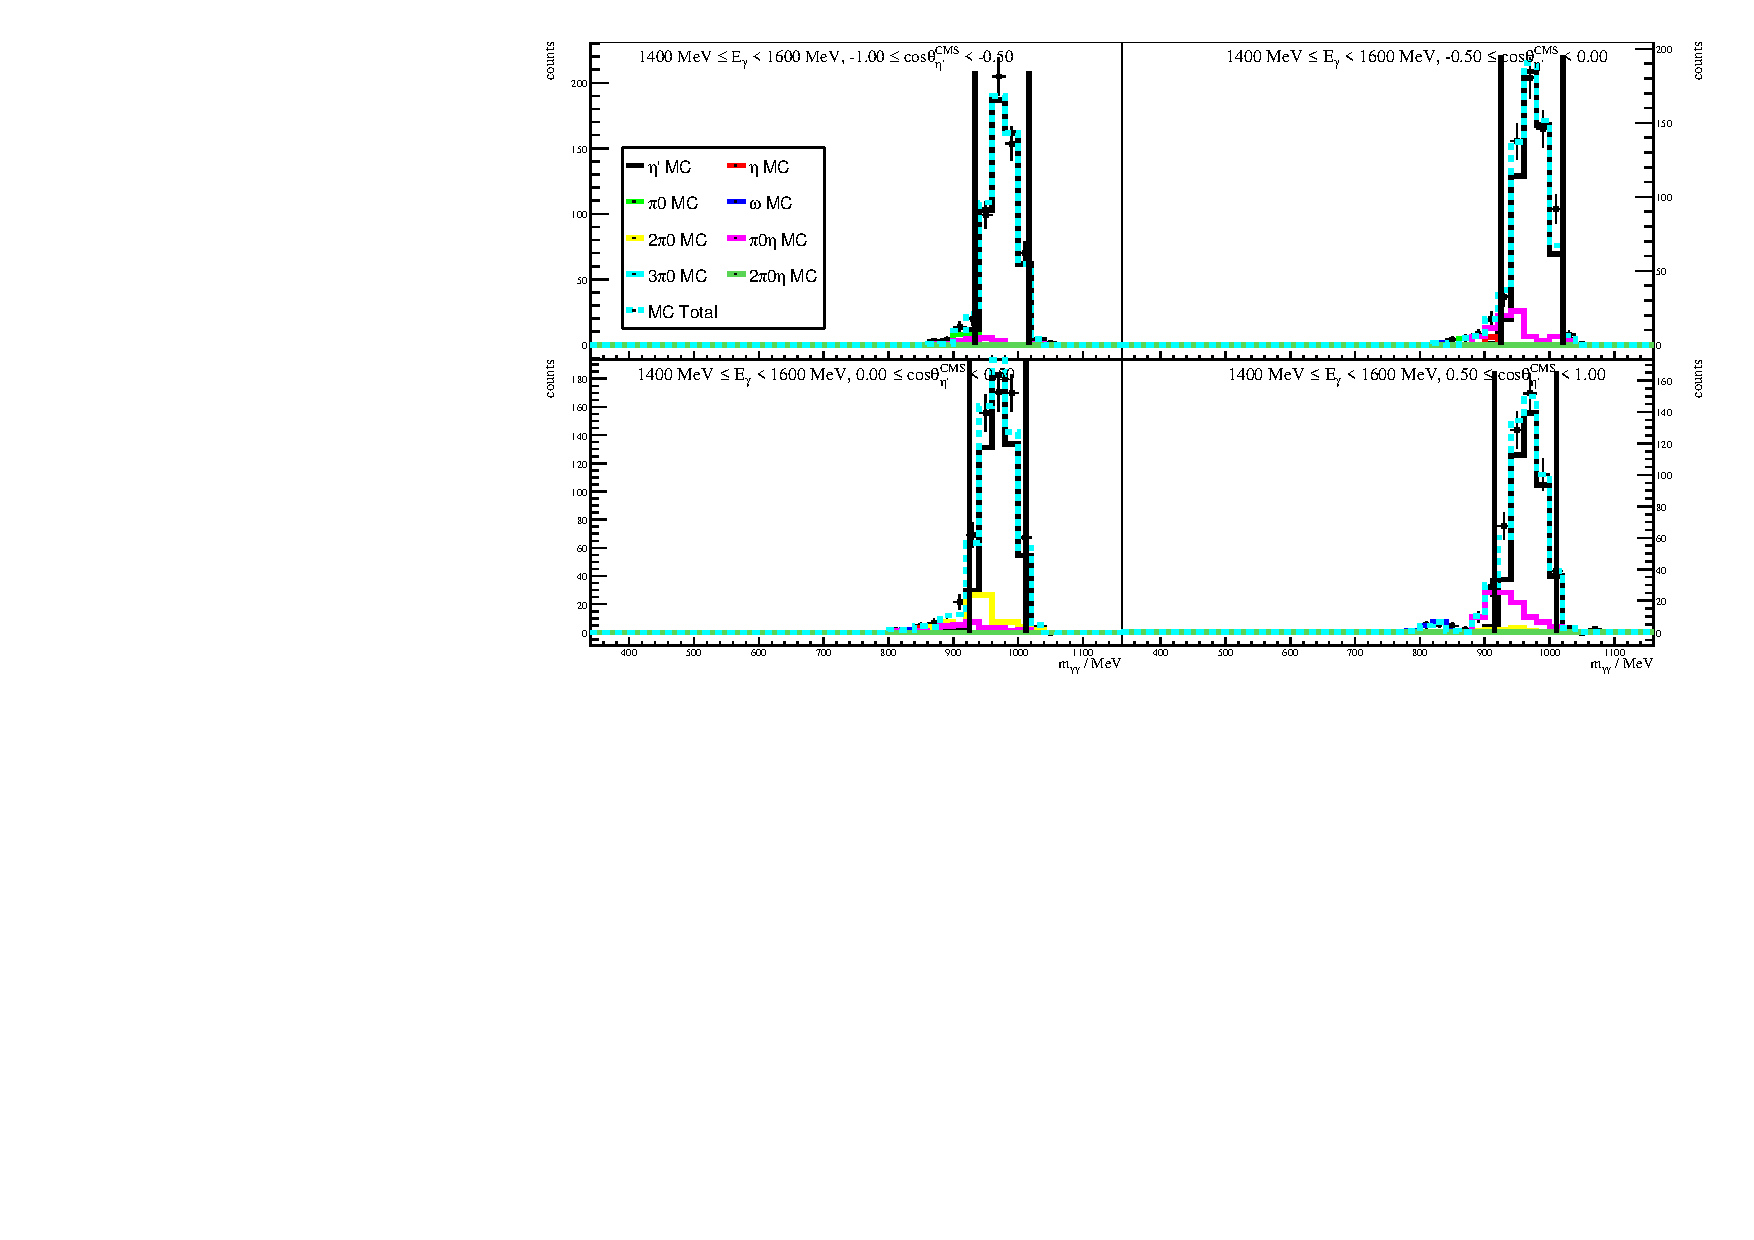
\includegraphics[width=\linewidth]{invcut_ebin0.pdf}
		\end{figure}
		
	\end{frame}
	\begin{frame}{Event selection}
		Additional cuts to (try to) reduce bkg: 
		\begin{itemize}
			\item $p$ in CB for $E_\gamma<1500$ MeV
			\item $E_{\gamma_{i}}<1500$ MeV
			\item ClusterPEDCount$(\gamma_i)=1$
			\item Clustersize$(p)<6$
			\item Clustersize ($\gamma_{i}$) in FW
		\end{itemize}
		\begin{figure}
			\centering
			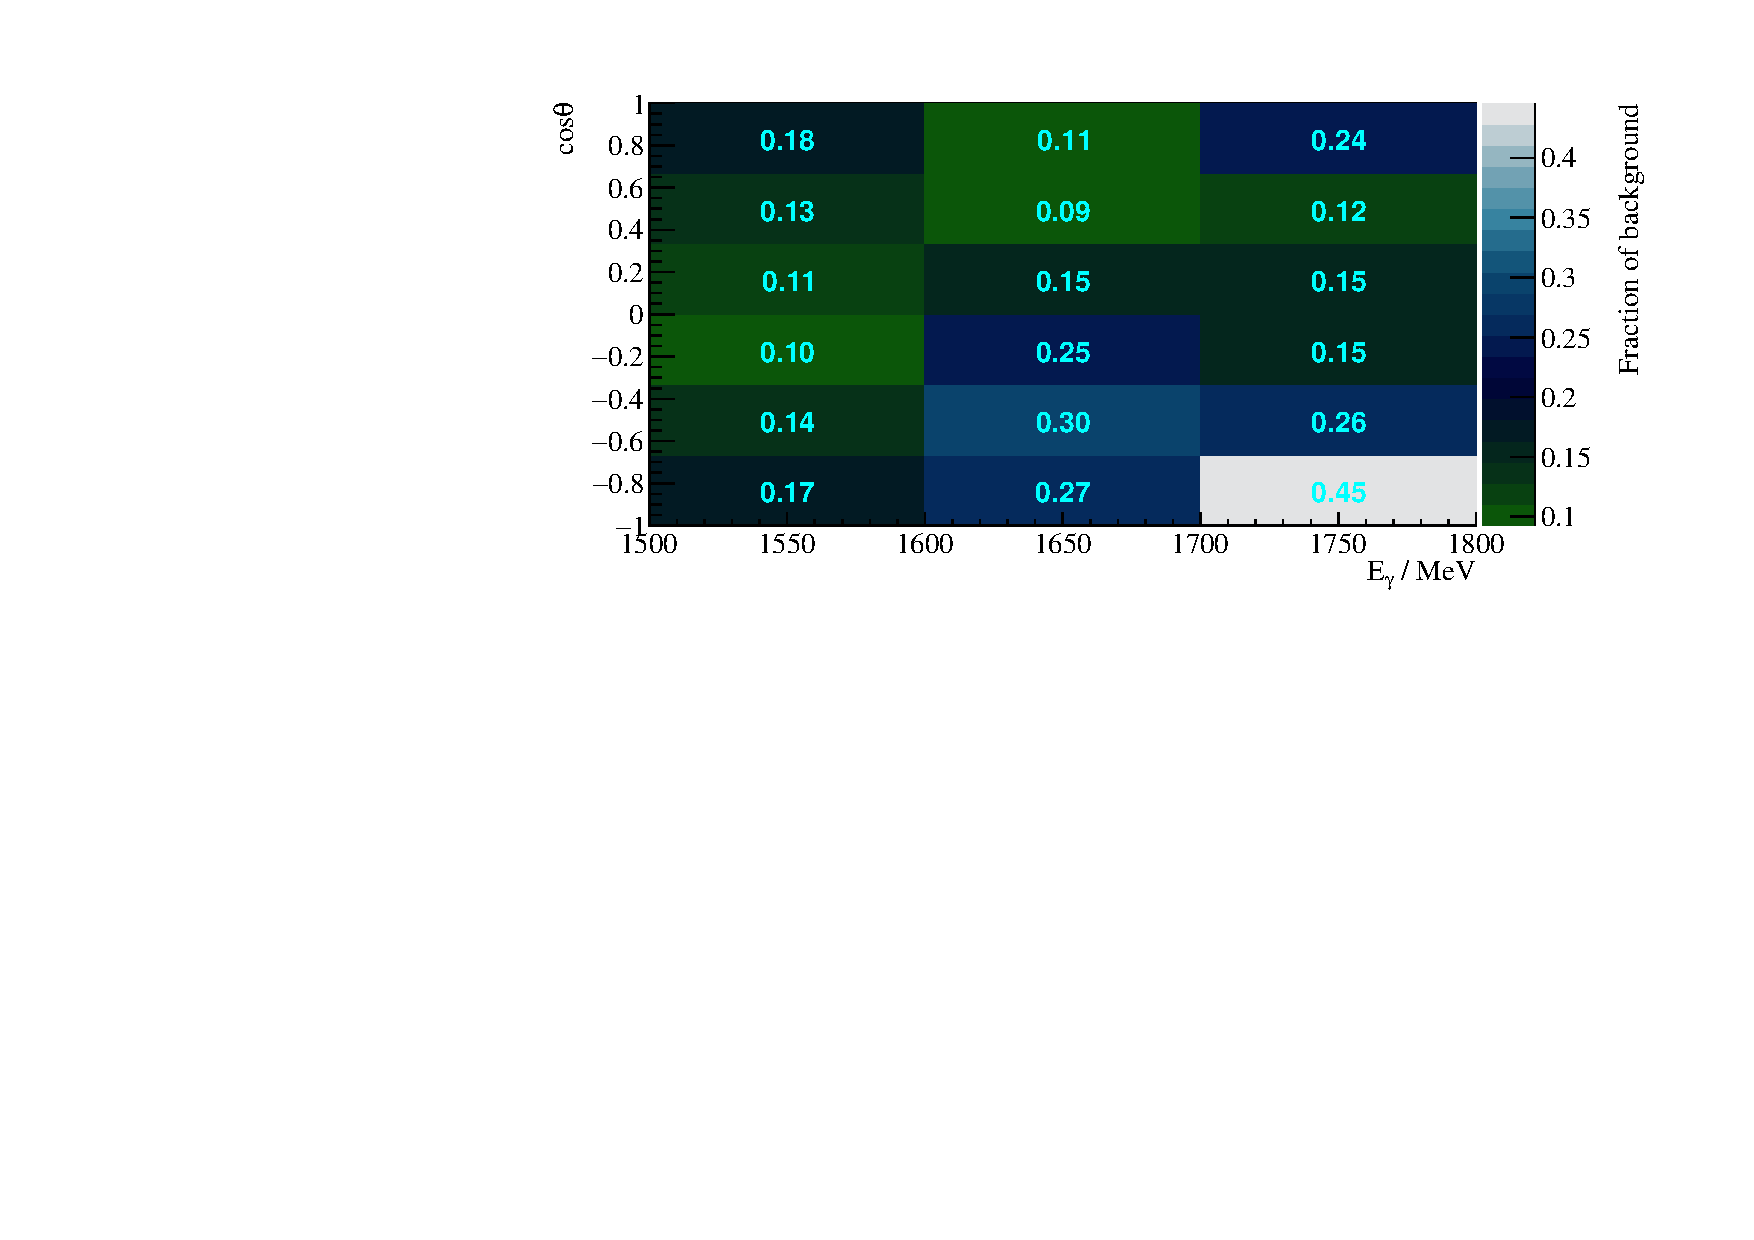
\includegraphics[width=.49\linewidth]{../../figs/hydrogen/bin_cuts/invcut_bkg_percentage.pdf}
			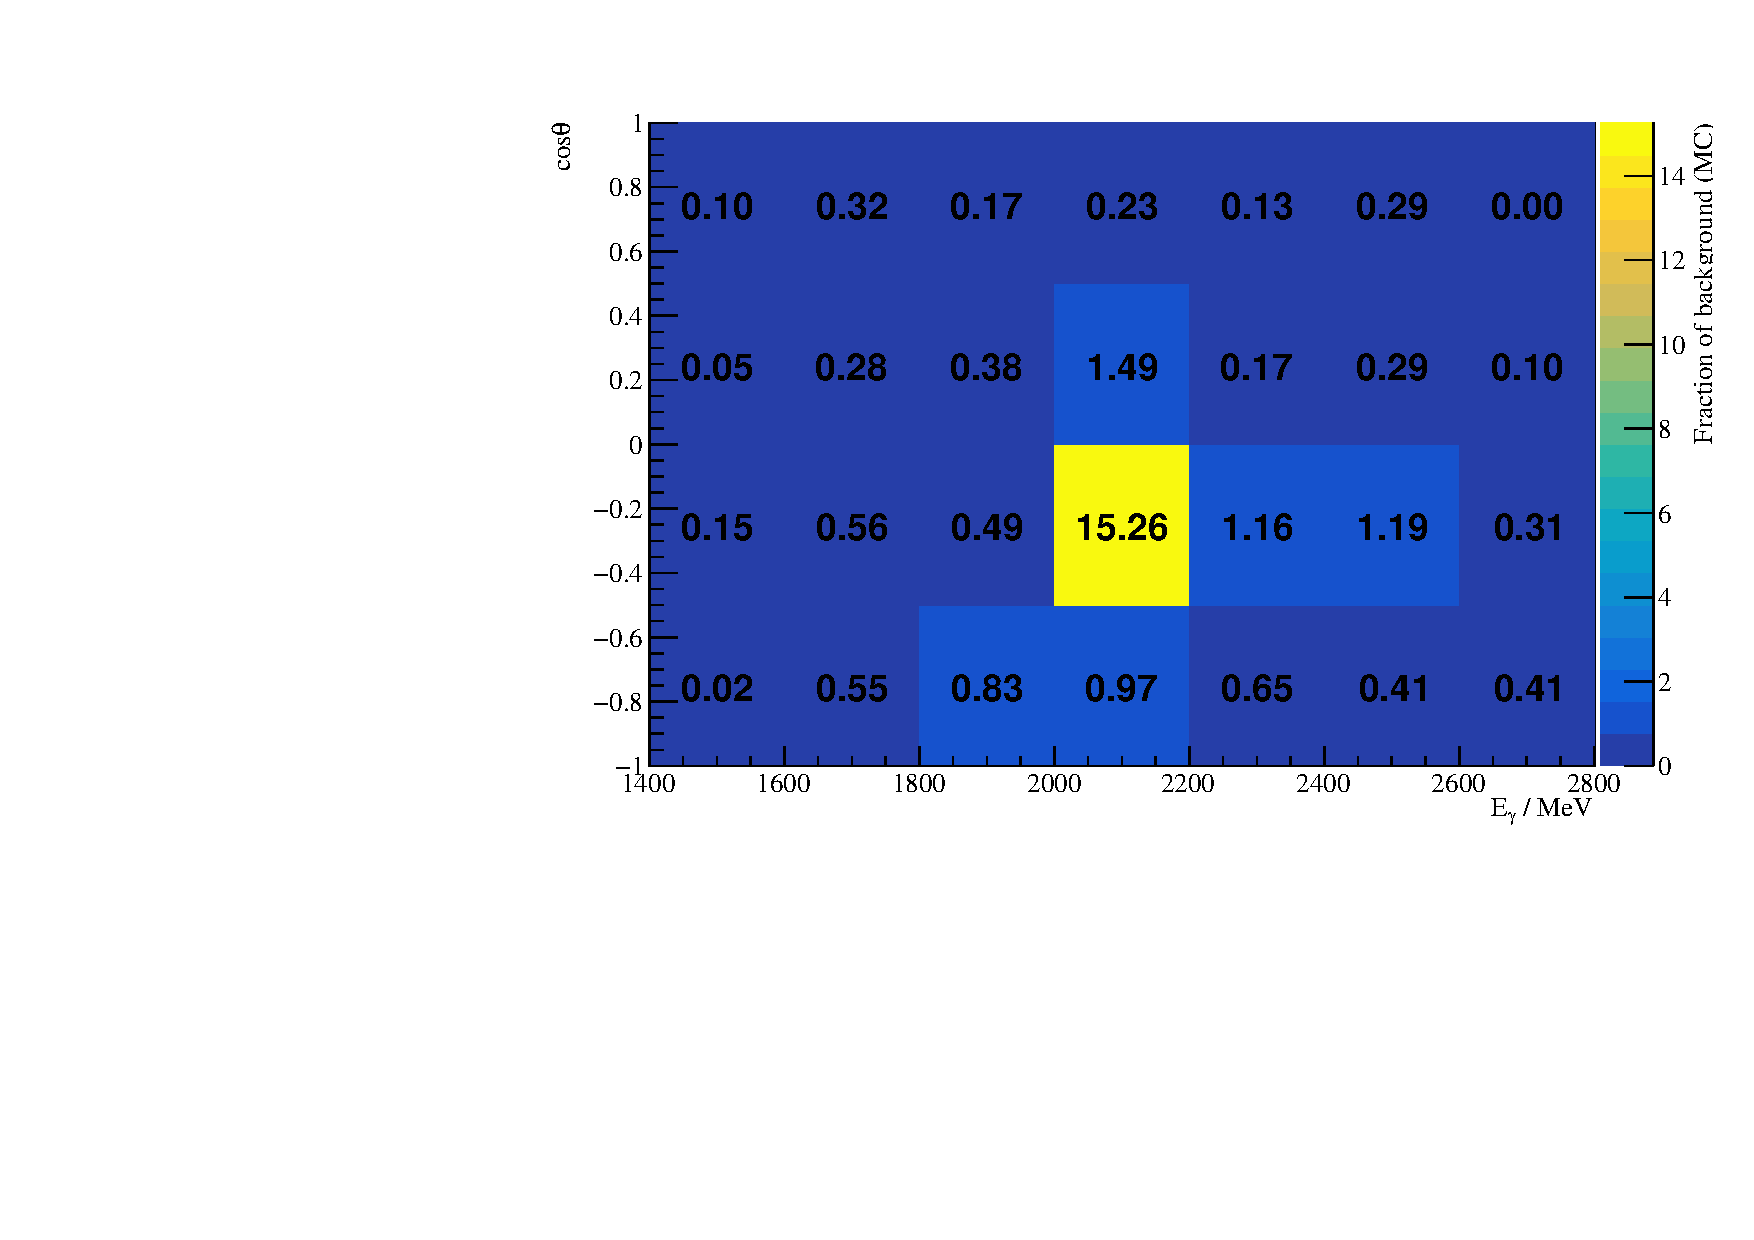
\includegraphics[width=.49\linewidth]{../../figs/hydrogen/bin_cuts_alt/invcut_bkg_percentage.pdf}
		\end{figure}
	\end{frame}
	\begin{frame}{Investigation of Background contributions ($2\pi^0\to4\gamma$ and $\pi^0\eta\to4\gamma$)}
	two cases: $E_\gamma\lesssim 20$ MeV, or $\theta_{\gamma_{i}}\approx\theta_{\gamma_{j}}$, combining two (or three) photons to one
	\begin{figure}
		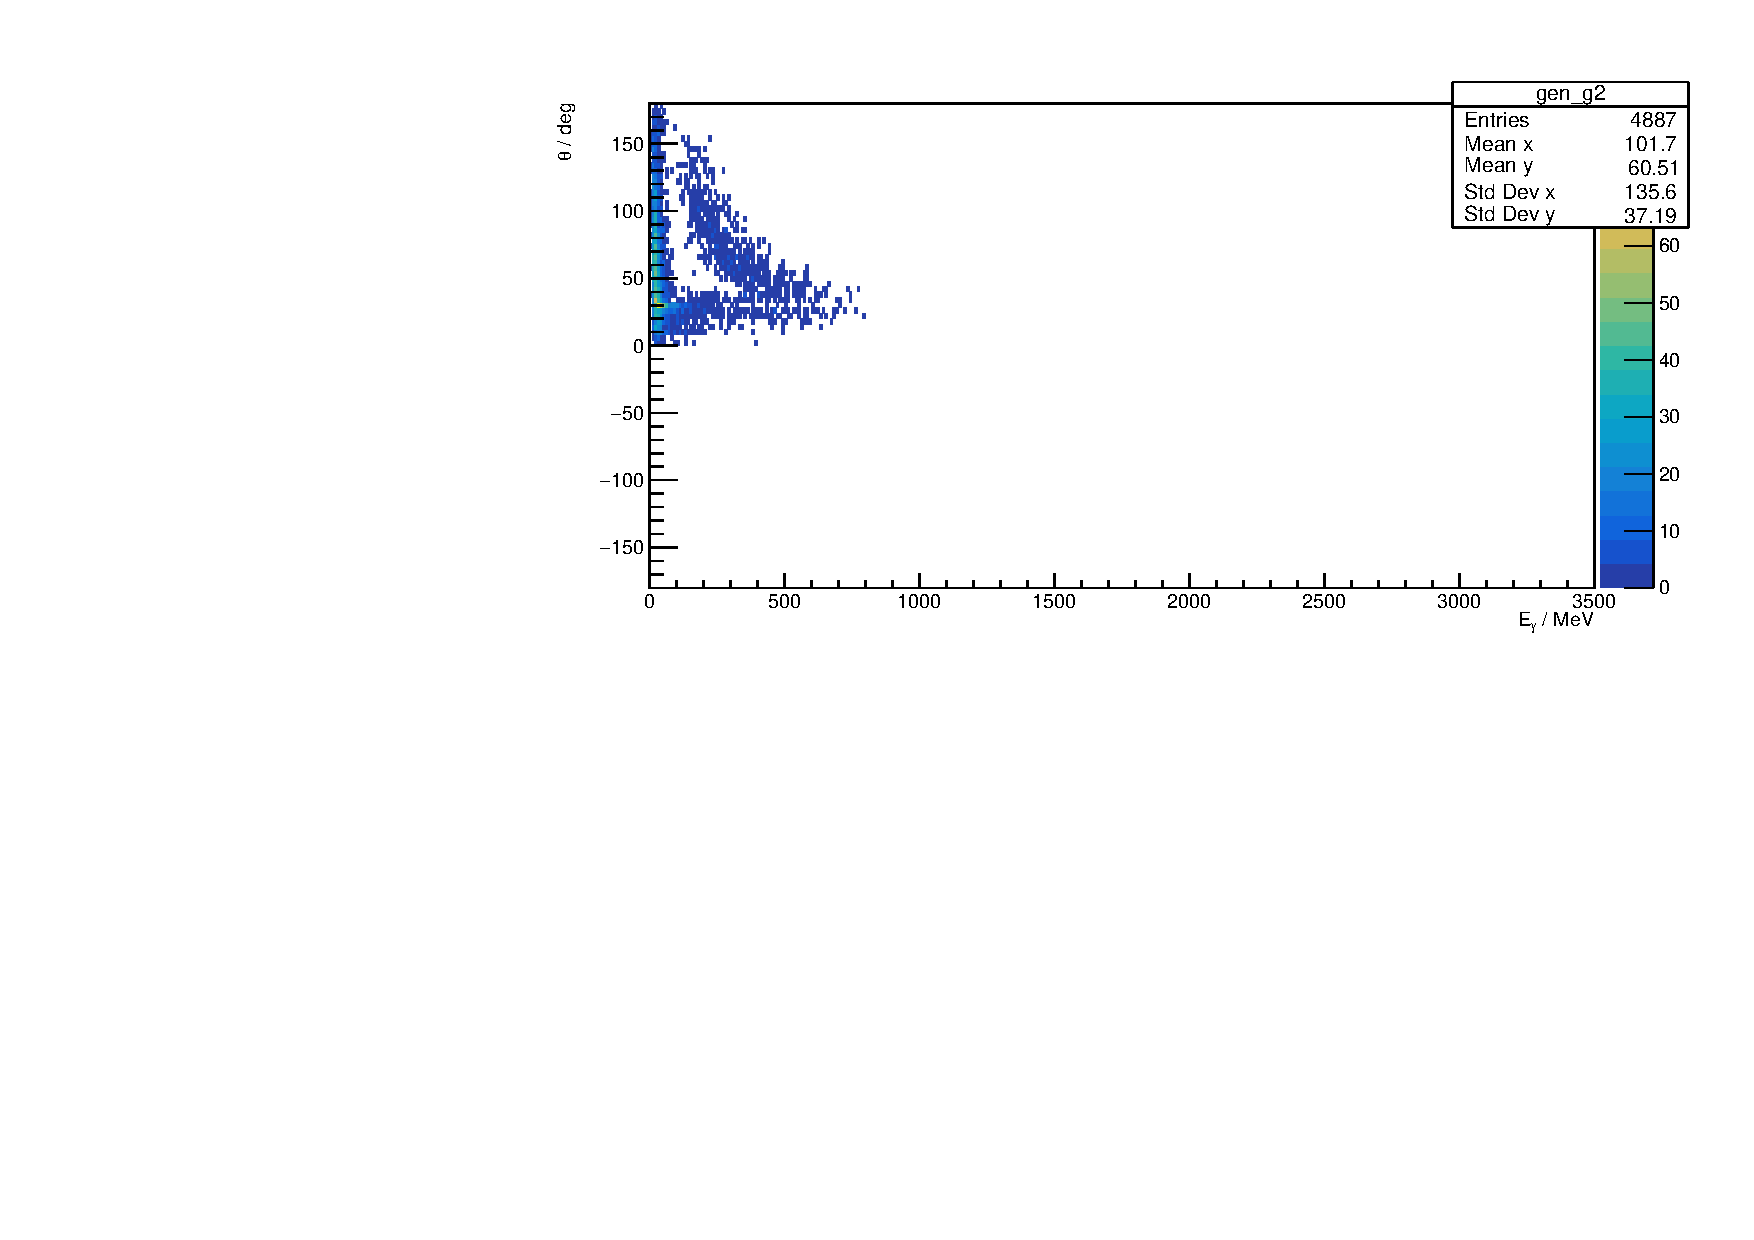
\includegraphics[width=.49\linewidth]{../../figs/hydrogen/gen_g2_2pi0.pdf}
		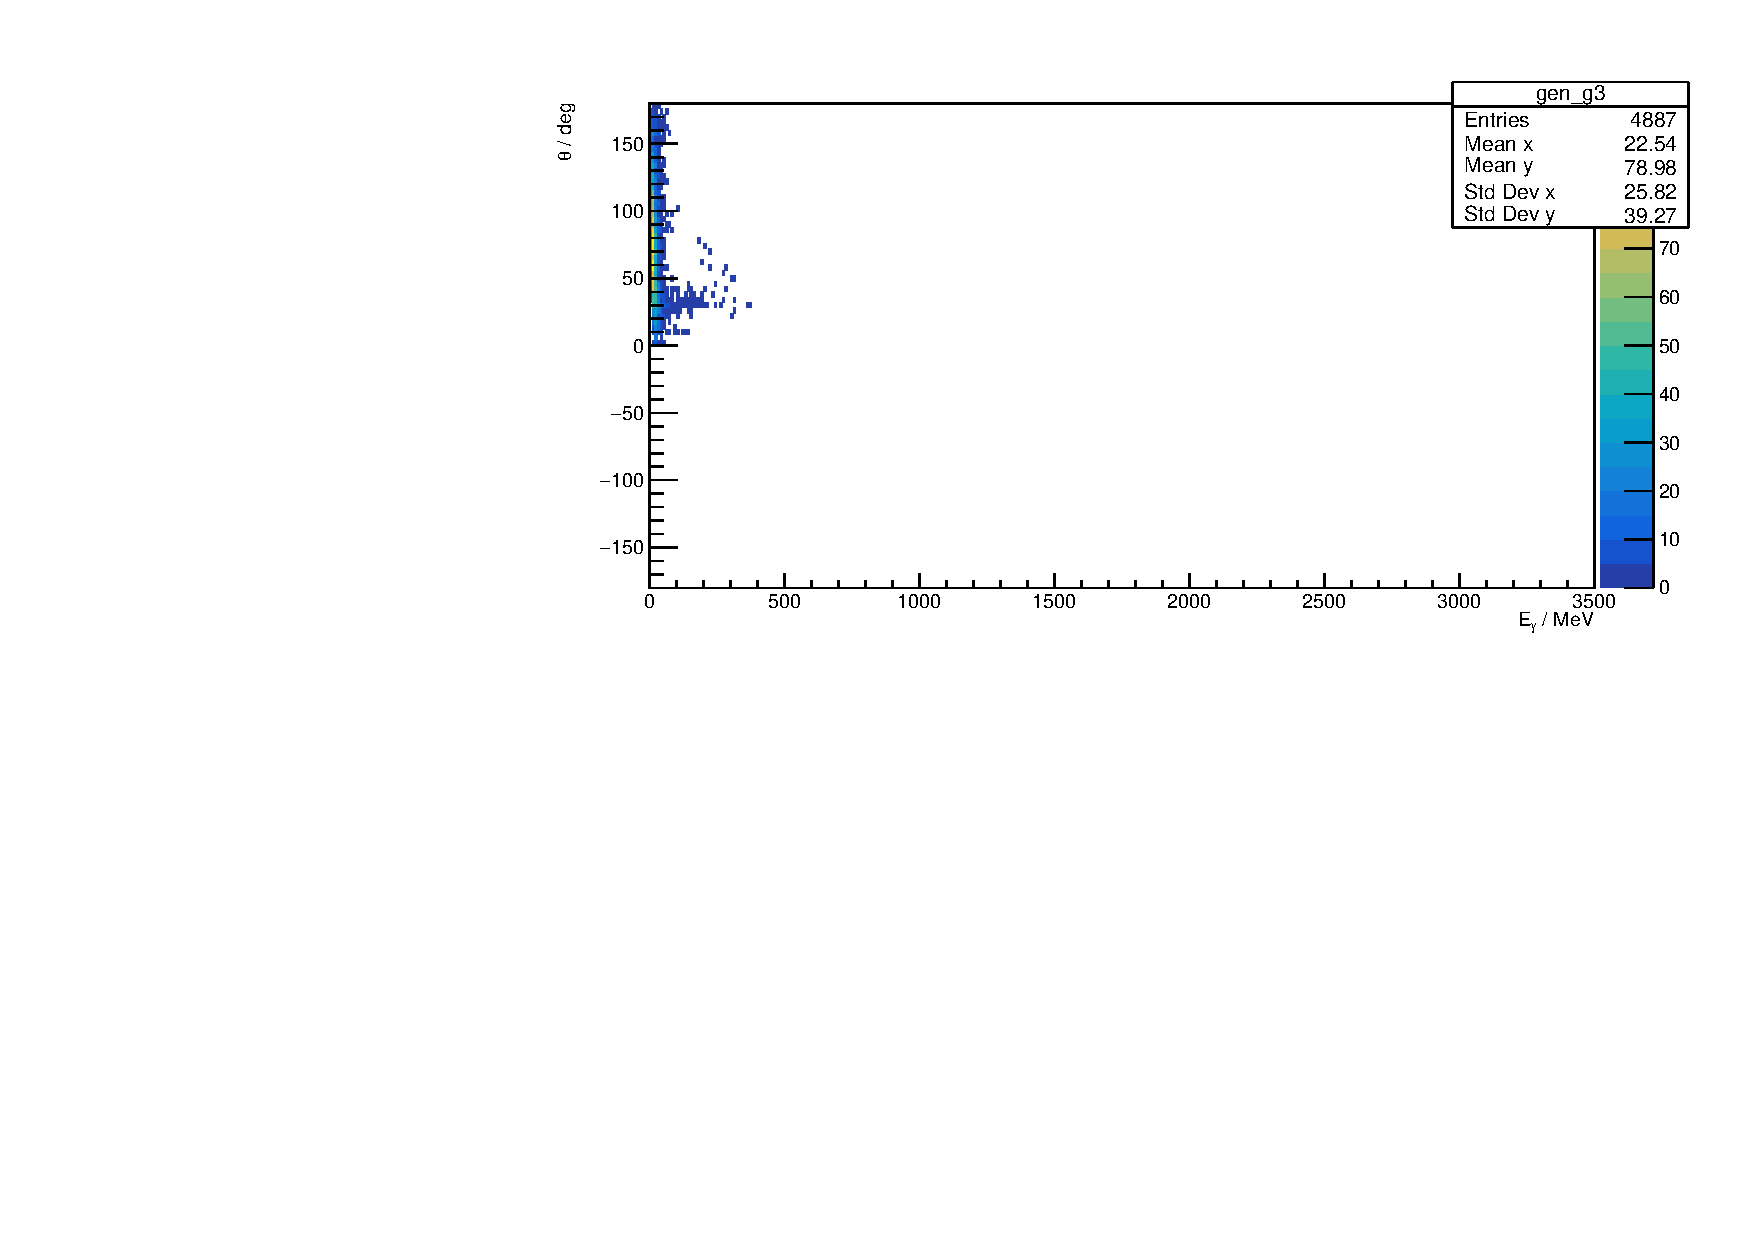
\includegraphics[width=.49\linewidth]{../../figs/hydrogen/gen_g3_2pi0.pdf}
		\caption*{Two lowest energy photons of $2\pi^0$ production (MC)}
	\end{figure}
	\end{frame}
	\begin{frame}{Investigation of Background contributions ($2\pi^0\to4\gamma$ and $\pi^0\eta\to4\gamma$)}
	\begin{figure}
		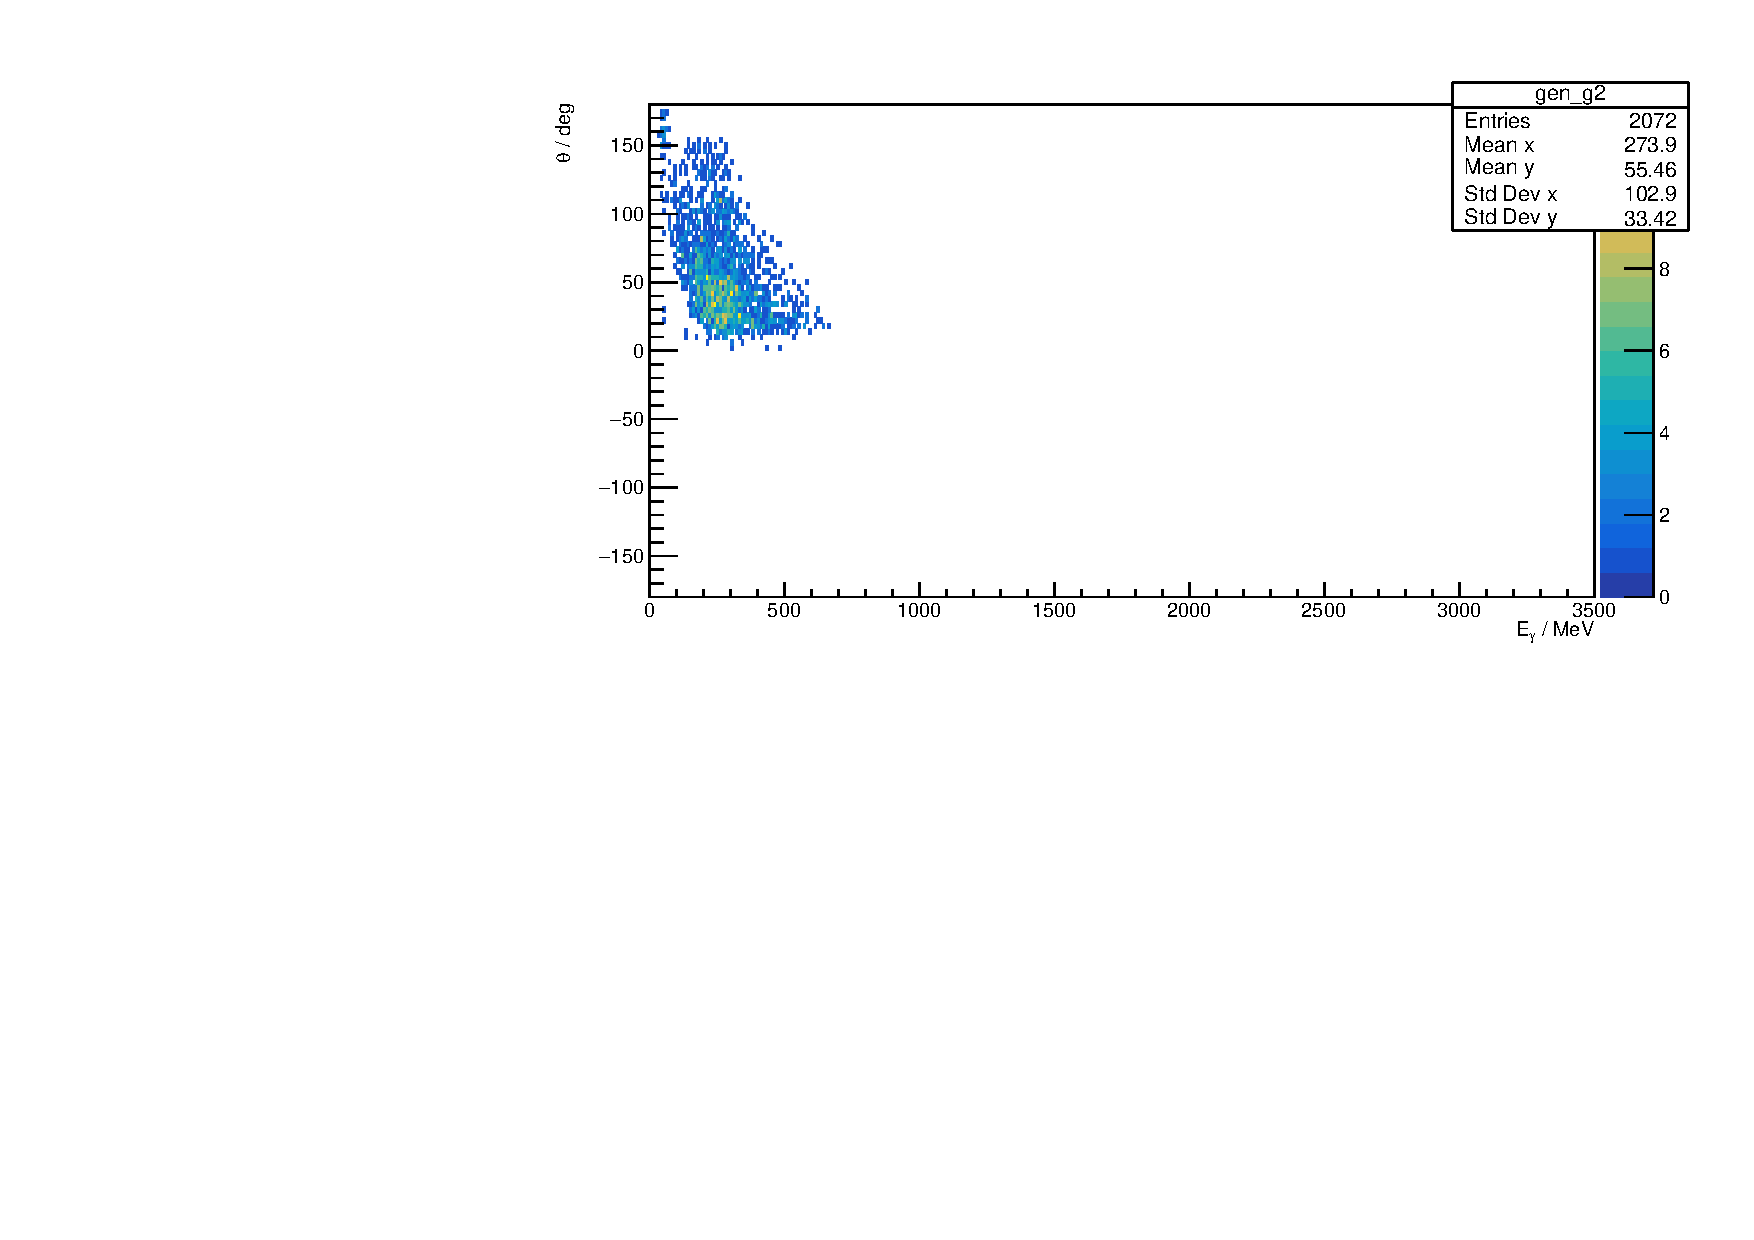
\includegraphics[width=.49\linewidth]{../../figs/hydrogen/gen_g2_pi0eta.pdf}
		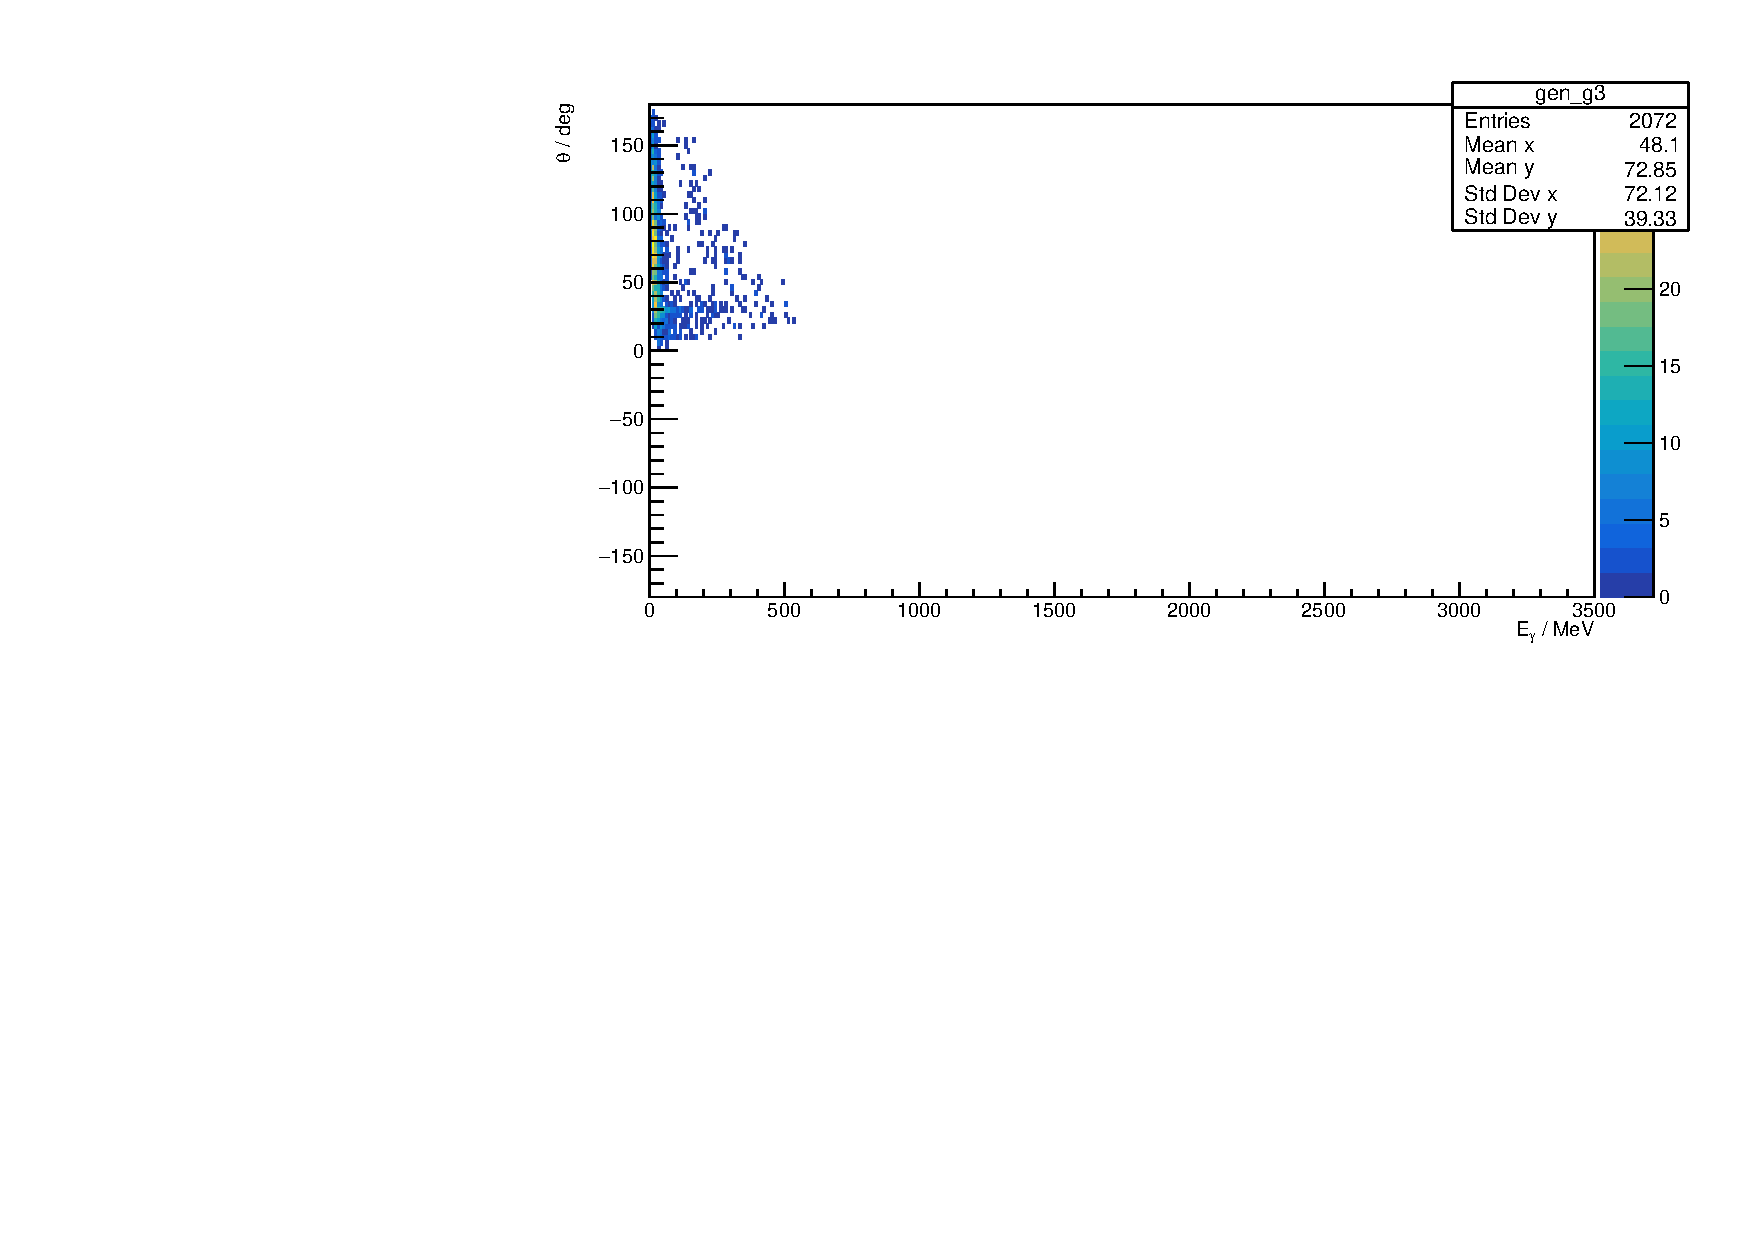
\includegraphics[width=.49\linewidth]{../../figs/hydrogen/gen_g3_pi0eta.pdf}
		\caption*{Two lowest energy photons of $\pi^0\eta$ production (MC)}
	\end{figure}
\end{frame}
\begin{frame}{Investigation of Background contributions ($2\pi^0\to4\gamma$ and $\pi^0\eta\to4\gamma$)}
	\begin{figure}
		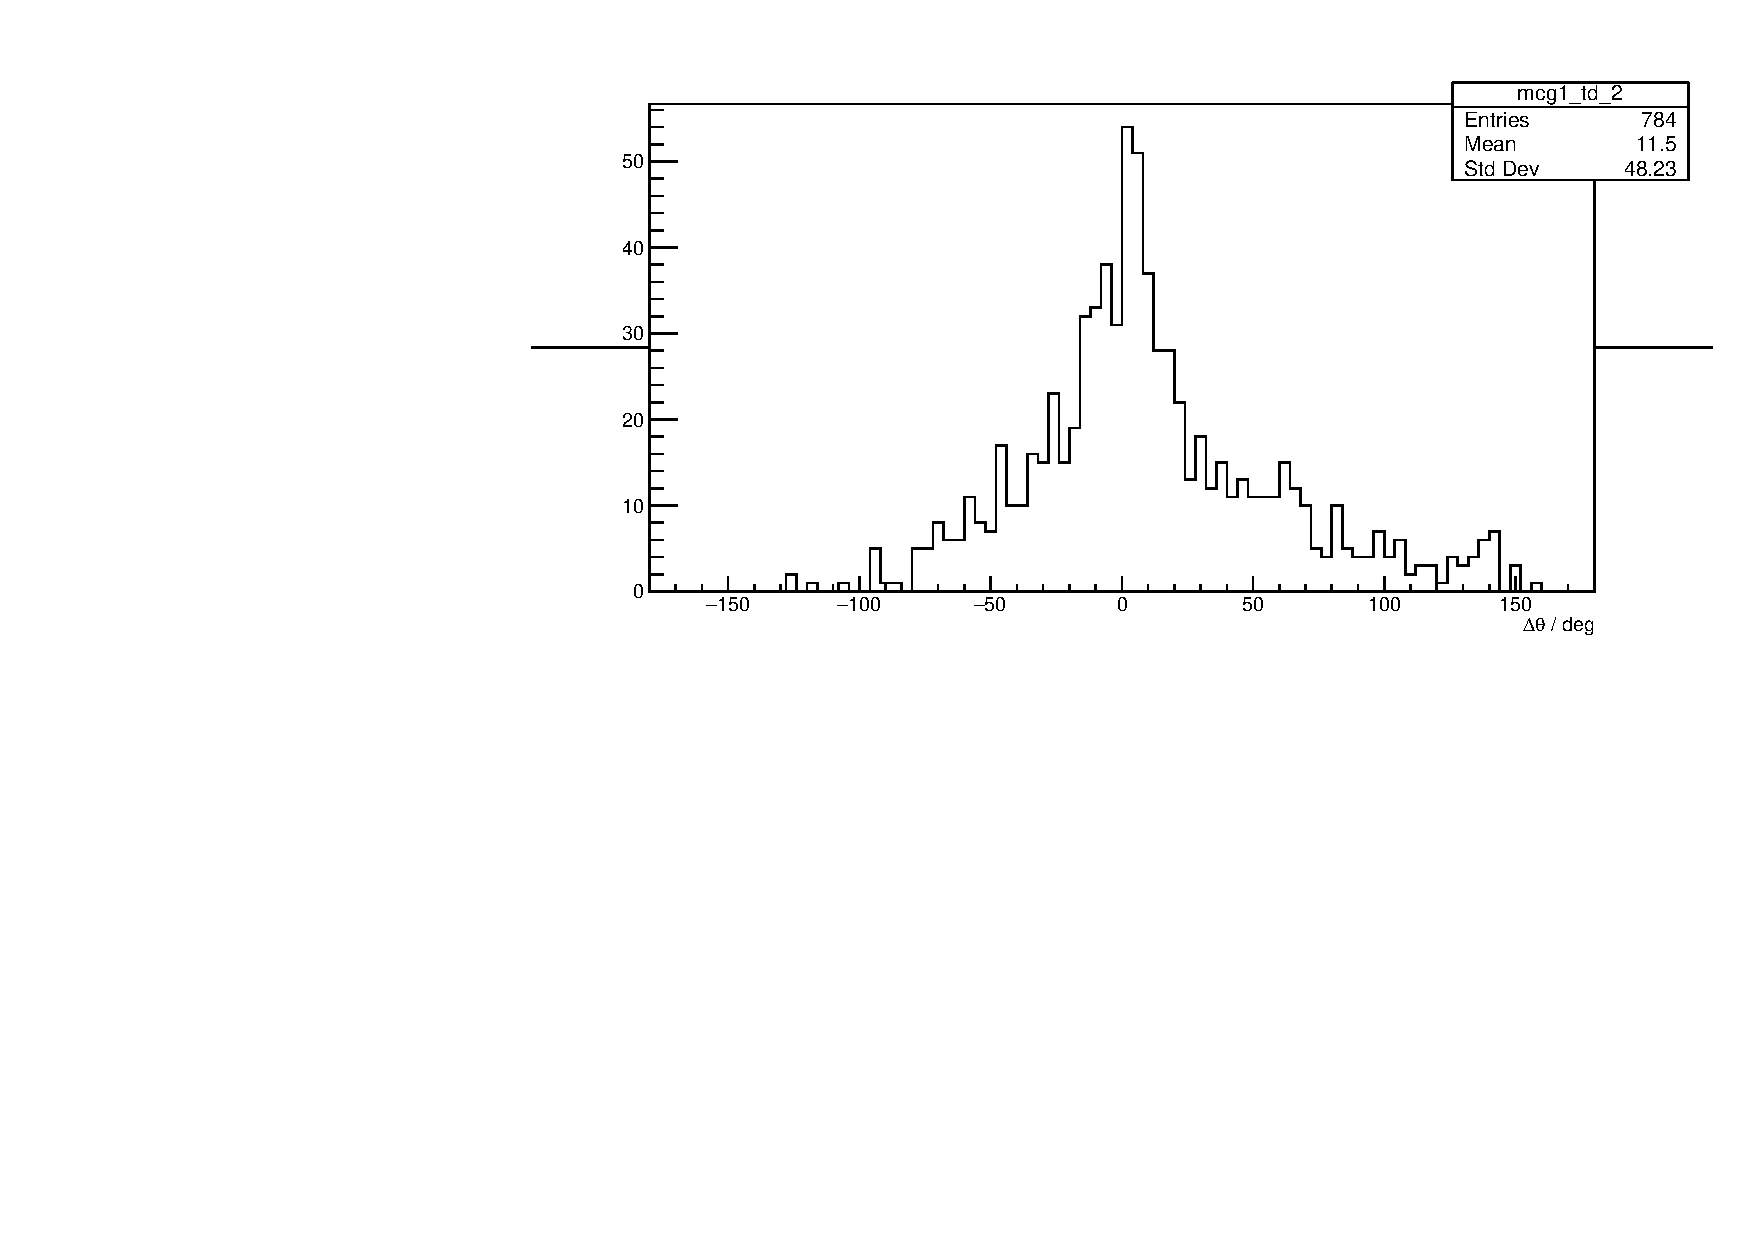
\includegraphics[width=.49\linewidth]{../../figs/hydrogen/mctd_2_2pi0.pdf}
		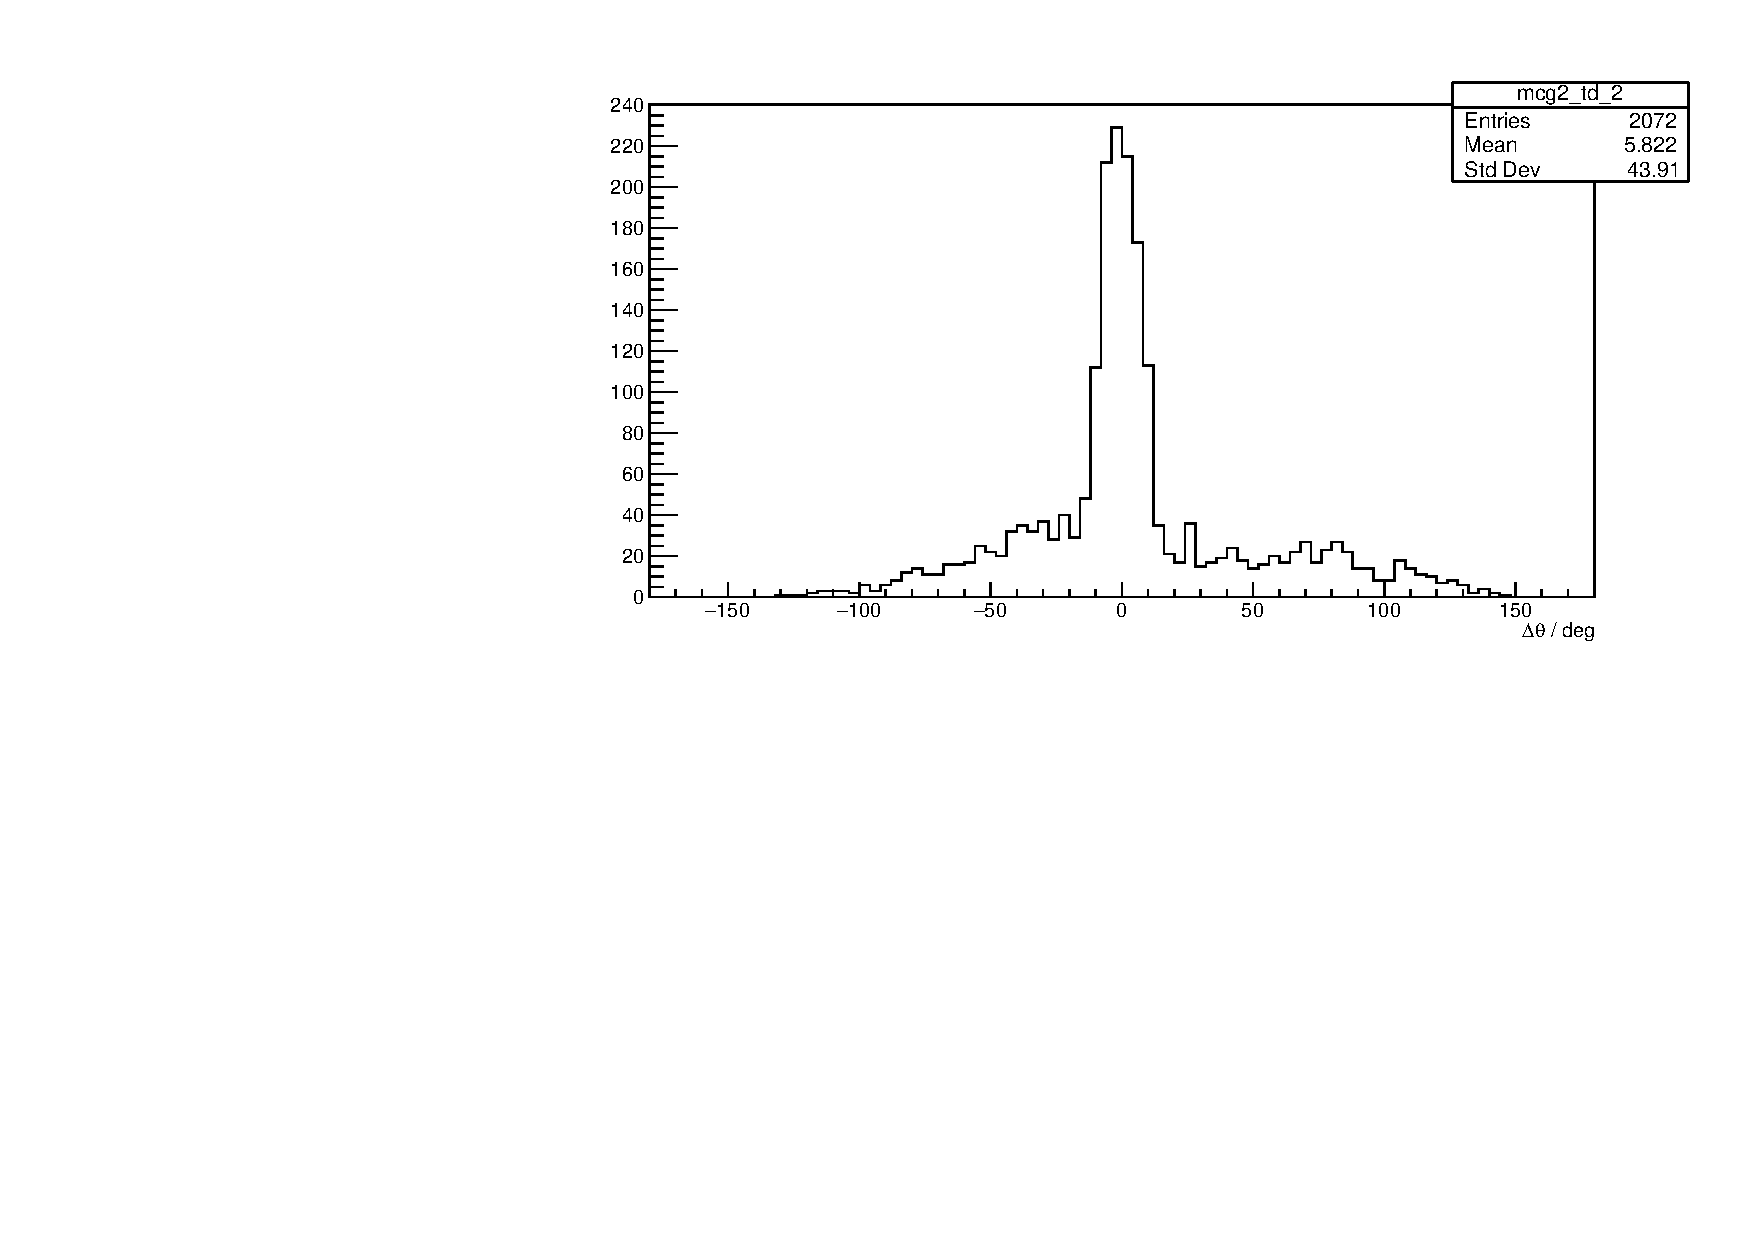
\includegraphics[width=.49\linewidth]{../../figs/hydrogen/mctd_2_pi0eta.pdf}
		\caption*{Angular difference between second lowest energy photon and one of the highest energy photons }
	\end{figure}
\end{frame}
\begin{frame}{Investigation of Background contributions ($2\pi^0\to4\gamma$ and $\pi^0\eta\to4\gamma$)}
	\begin{figure}
		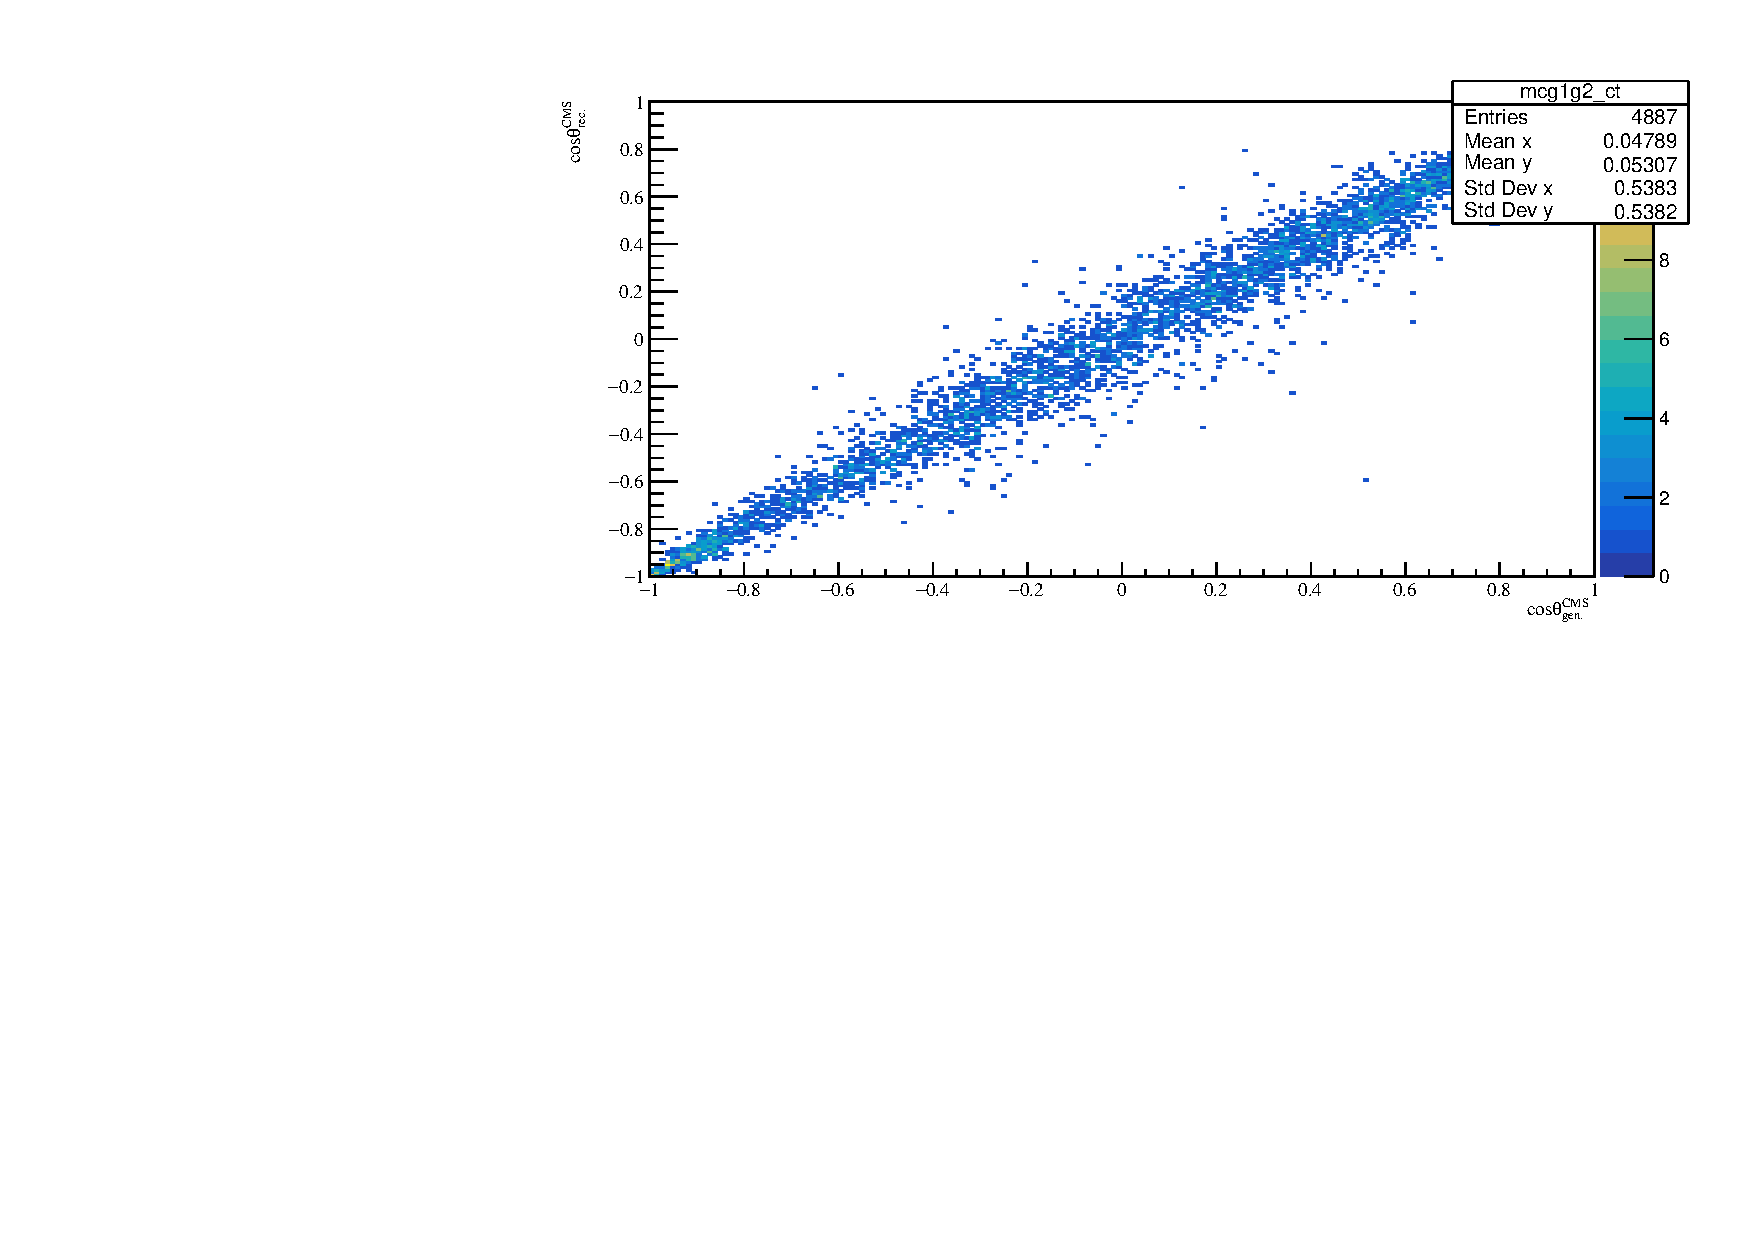
\includegraphics[width=.49\linewidth]{../../figs/hydrogen/costheta_2pi0.pdf}
		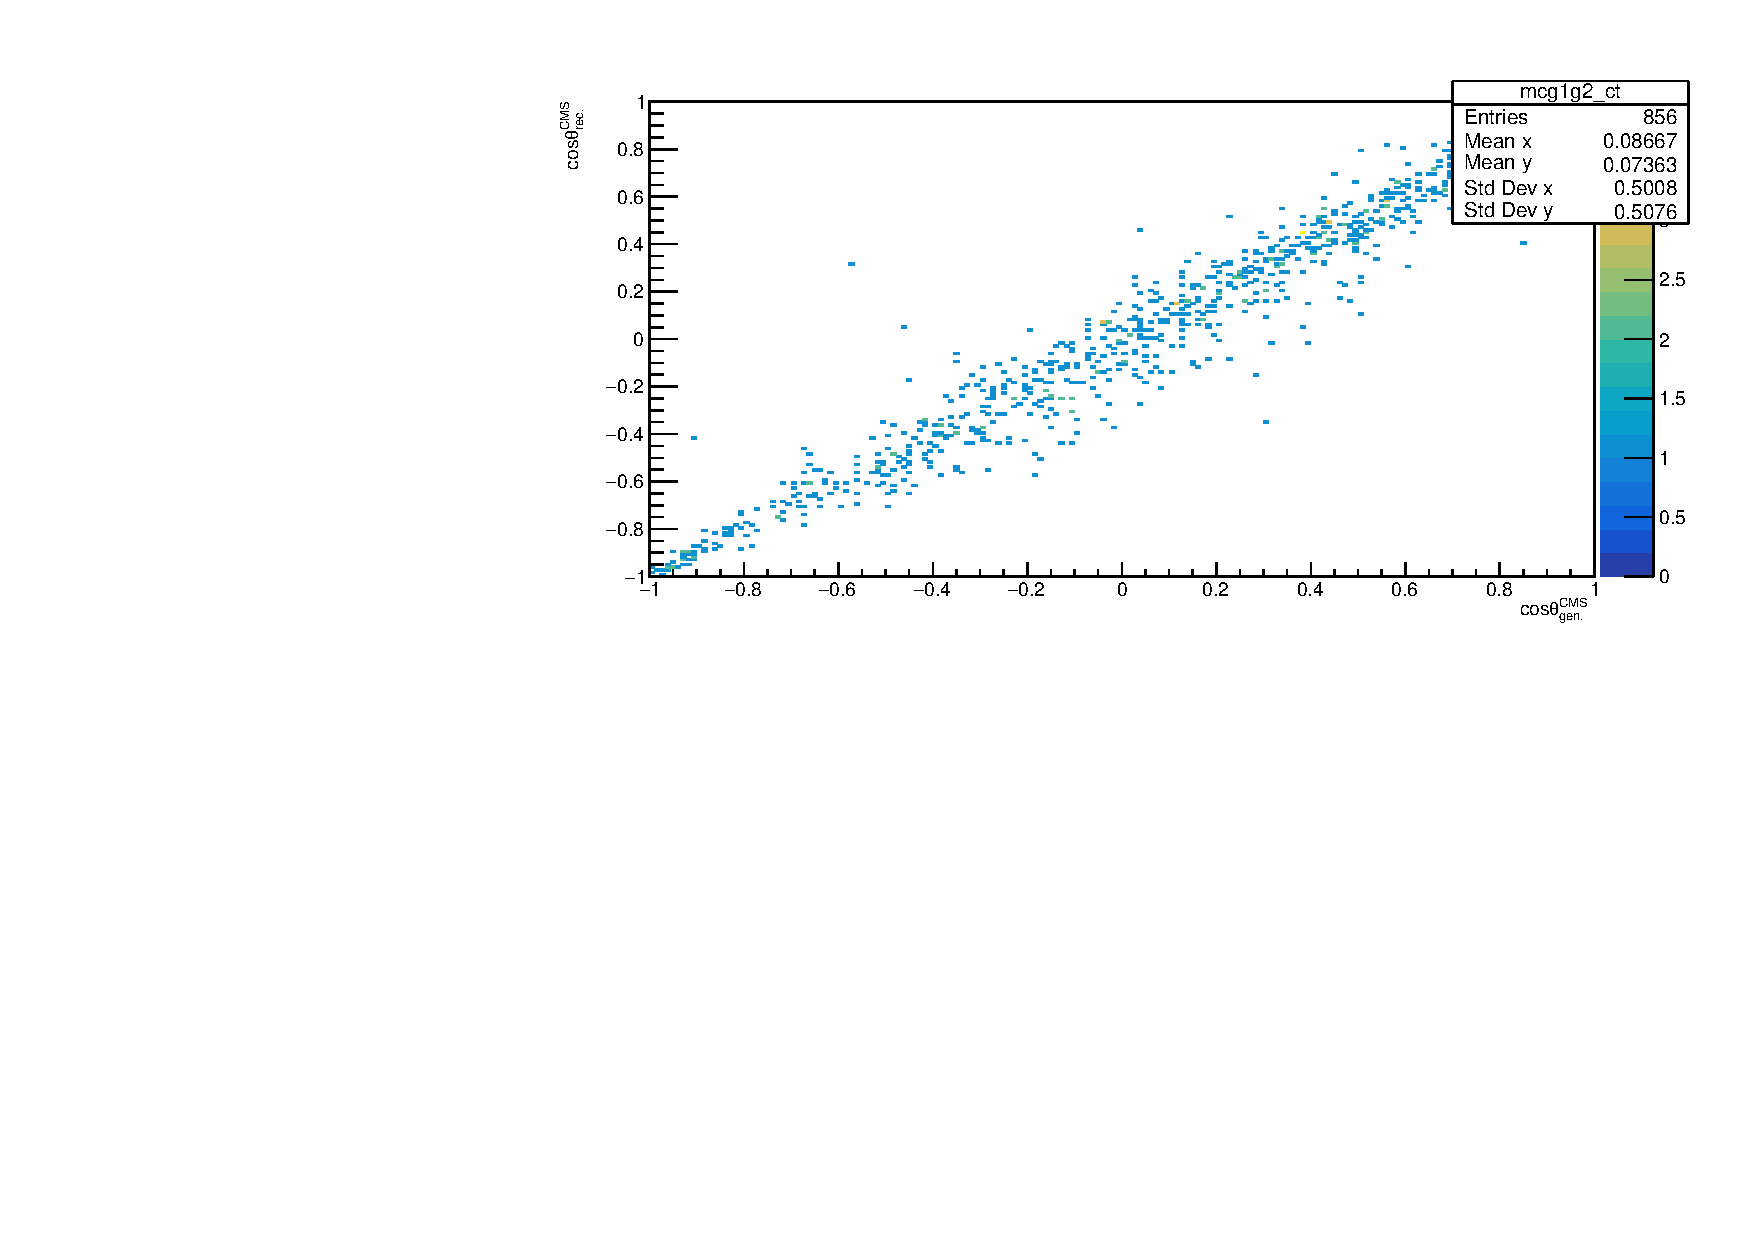
\includegraphics[width=.49\linewidth]{../../figs/hydrogen/costheta_pi0eta.pdf}
		\caption*{gen. CMS angle vs. meas. CMS angle for background contributions}
	\end{figure}
\end{frame}
	\begin{frame}{Asymmetry $A(\phi)=\frac{N^\bot-N^\parallel}{p_\gamma^\parallel N^\bot+p_\gamma^\bot N^\parallel}=\Sigma \cos\left(2\left(\alpha^\parallel-\phi\right)\right)$ }
		\begin{figure}
			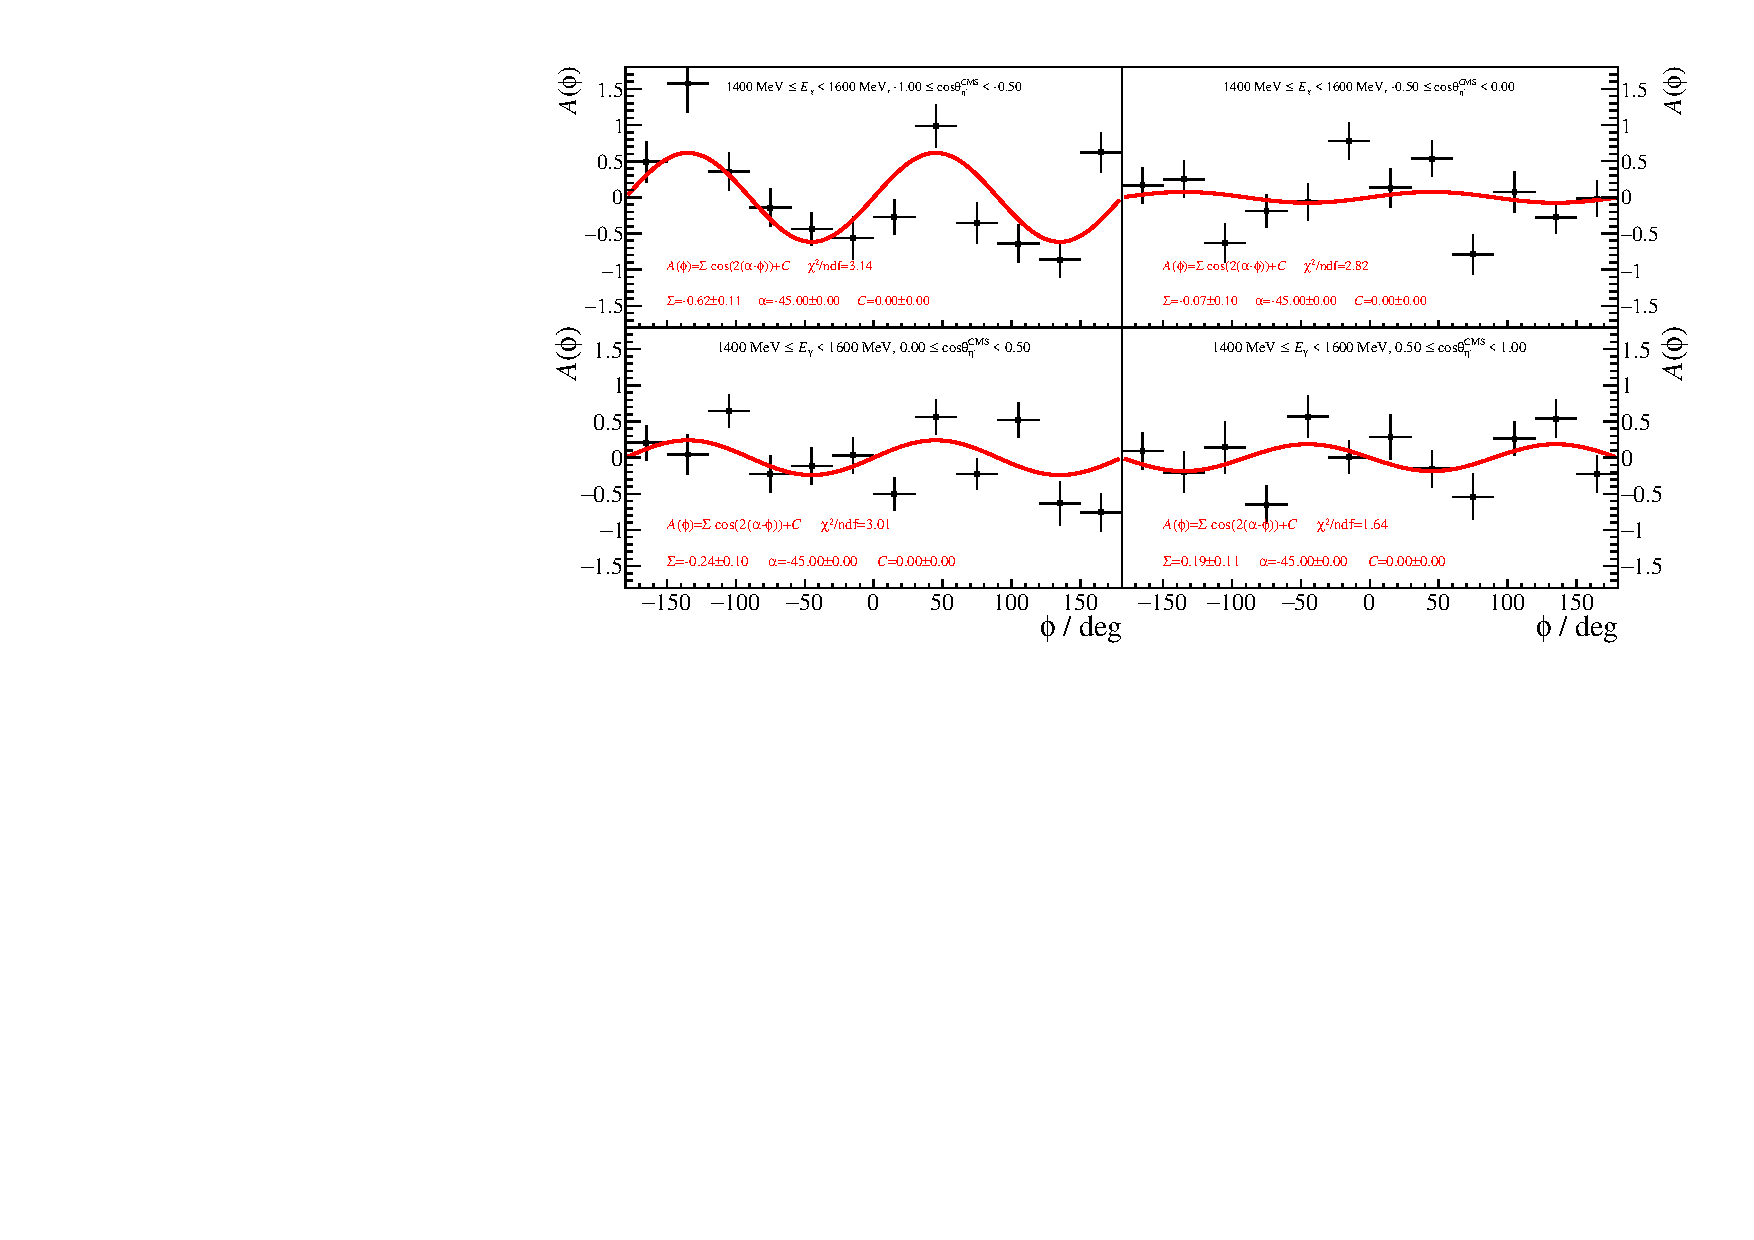
\includegraphics[width=\linewidth]{../../figs/hydrogen/asymmetry/ebin_0_fixalphaC.pdf}
		\end{figure}
	\end{frame}
	\begin{frame}{Beam asymmetry $\Sigma$}
		\begin{figure}
			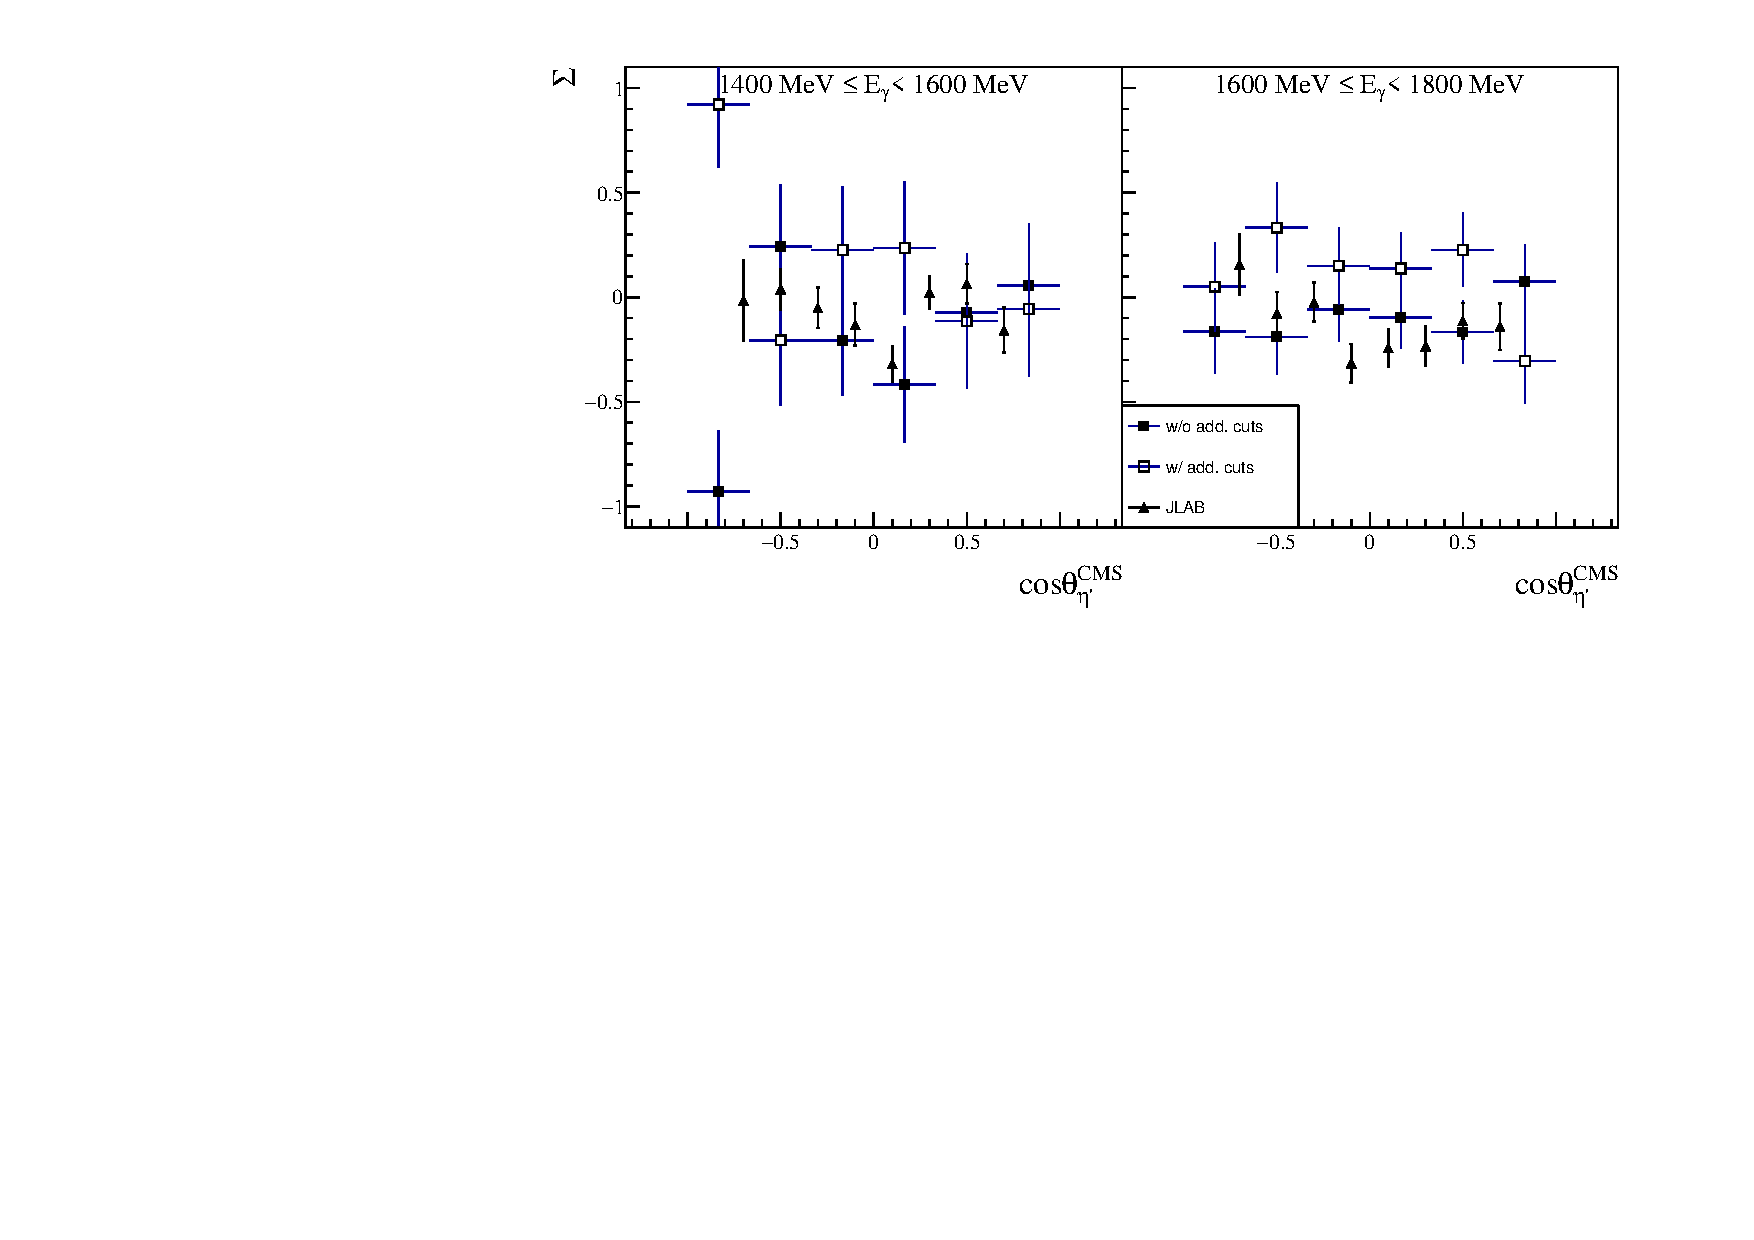
\includegraphics[width=\linewidth]{../../figs/hydrogen/asymmetry/sigma.pdf}
		\end{figure}
	\end{frame}
\end{document}
